% This file was created by matlab2tikz.
%
%The latest updates can be retrieved from
%  http://www.mathworks.com/matlabcentral/fileexchange/22022-matlab2tikz-matlab2tikz
%where you can also make suggestions and rate matlab2tikz.
%

\pgfplotsset{compat=newest}

\usetikzlibrary{calc}

%%% START MACRO FOR ANNOTATION OF TRIANGLE WITH SLOPE %%%.
\newcommand{\logLogSlopeTriangle}[5]
{
	% #1. Relative offset in x direction.
	% #2. Width in x direction, so xA-xB.
	% #3. Relative offset in y direction.
	% #4. Slope d(y)/d(log10(x)).
	% #5. Plot options.
	
	\pgfplotsextra
	{
		\pgfkeysgetvalue{/pgfplots/xmin}{\xmin}
		\pgfkeysgetvalue{/pgfplots/xmax}{\xmax}
		\pgfkeysgetvalue{/pgfplots/ymin}{\ymin}
		\pgfkeysgetvalue{/pgfplots/ymax}{\ymax}
		
		% Calculate auxilliary quantities, in relative sense.
		\pgfmathsetmacro{\xArel}{#1}
		\pgfmathsetmacro{\yArel}{#3}
		\pgfmathsetmacro{\xBrel}{#1-#2}
		\pgfmathsetmacro{\yBrel}{\yArel}
		\pgfmathsetmacro{\xCrel}{\xArel}
		%\pgfmathsetmacro{\yCrel}{ln(\yC/exp(\ymin))/ln(exp(\ymax)/exp(\ymin))} % REPLACE THIS EXPRESSION WITH AN EXPRESSION INDEPENDENT OF \yC TO PREVENT THE 'DIMENSION TOO LARGE' ERROR.
		
		\pgfmathsetmacro{\lnxB}{\xmin*(1-(#1-#2))+\xmax*(#1-#2)} % in [xmin,xmax].
		\pgfmathsetmacro{\lnxA}{\xmin*(1-#1)+\xmax*#1} % in [xmin,xmax].
		\pgfmathsetmacro{\lnyA}{\ymin*(1-#3)+\ymax*#3} % in [ymin,ymax].
		\pgfmathsetmacro{\lnyC}{\lnyA-#4*(\lnxA-\lnxB)}
		\pgfmathsetmacro{\yCrel}{\lnyC-\ymin)/(\ymax-\ymin)}
		
		% Define coordinates for \draw. MIND THE 'rel axis cs' as opposed to the 'axis cs'.
		\coordinate (A) at (rel axis cs:\xArel,\yArel);
		\coordinate (B) at (rel axis cs:\xBrel,\yBrel);
		\coordinate (C) at (rel axis cs:\xCrel,\yCrel);
		
		% Draw slope triangle.
		\draw[#5]   (A)-- node[pos=0.5,anchor=south] {\scriptsize 1}
		(B)-- 
		(C)-- node[pos=0.5,anchor=west] {\scriptsize #4}
		cycle;
	}
}

\newcommand{\logLogSlopeReverseTriangle}[5]
{
	% #1. Relative offset in x direction.
	% #2. Width in x direction, so xA-xB.
	% #3. Relative offset in y direction.
	% #4. Slope d(y)/d(log10(x)).
	% #5. Plot options.
	
	\pgfplotsextra
	{
		\pgfkeysgetvalue{/pgfplots/xmin}{\xmin}
		\pgfkeysgetvalue{/pgfplots/xmax}{\xmax}
		\pgfkeysgetvalue{/pgfplots/ymin}{\ymin}
		\pgfkeysgetvalue{/pgfplots/ymax}{\ymax}
		
		% Calculate auxilliary quantities, in relative sense.
		\pgfmathsetmacro{\xArel}{#1}
		\pgfmathsetmacro{\yArel}{#3}
		\pgfmathsetmacro{\xBrel}{#1+#2}
		\pgfmathsetmacro{\yBrel}{\yArel}
		\pgfmathsetmacro{\xCrel}{\xArel}
		%\pgfmathsetmacro{\yCrel}{ln(\yC/exp(\ymin))/ln(exp(\ymax)/exp(\ymin))} % REPLACE THIS EXPRESSION WITH AN EXPRESSION INDEPENDENT OF \yC TO PREVENT THE 'DIMENSION TOO LARGE' ERROR.
		
		\pgfmathsetmacro{\lnxB}{\xmin*(1-(#1-#2))+\xmax*(#1-#2)} % in [xmin,xmax].
		\pgfmathsetmacro{\lnxA}{\xmin*(1-#1)+\xmax*#1} % in [xmin,xmax].
		\pgfmathsetmacro{\lnyA}{\ymin*(1-#3)+\ymax*#3} % in [ymin,ymax].
		\pgfmathsetmacro{\lnyC}{\lnyA+#4*(\lnxA-\lnxB)}
		\pgfmathsetmacro{\yCrel}{\lnyC-\ymin)/(\ymax-\ymin)}
		
		% Define coordinates for \draw. MIND THE 'rel axis cs' as opposed to the 'axis cs'.
		\coordinate (A) at (rel axis cs:\xArel,\yArel);
		\coordinate (B) at (rel axis cs:\xBrel,\yBrel);
		\coordinate (C) at (rel axis cs:\xCrel,\yCrel);
		
		% Draw slope triangle.
		\draw[#5]   (A)-- node[pos=0.5,anchor=north] {\scriptsize 1}
		(B)-- 
		(C)-- node[pos=0.5,anchor=east] {\scriptsize #4}
		cycle;
	}
}
%%% END MACRO FOR ANNOTATION OF TRIANGLE WITH SLOPE %%%.


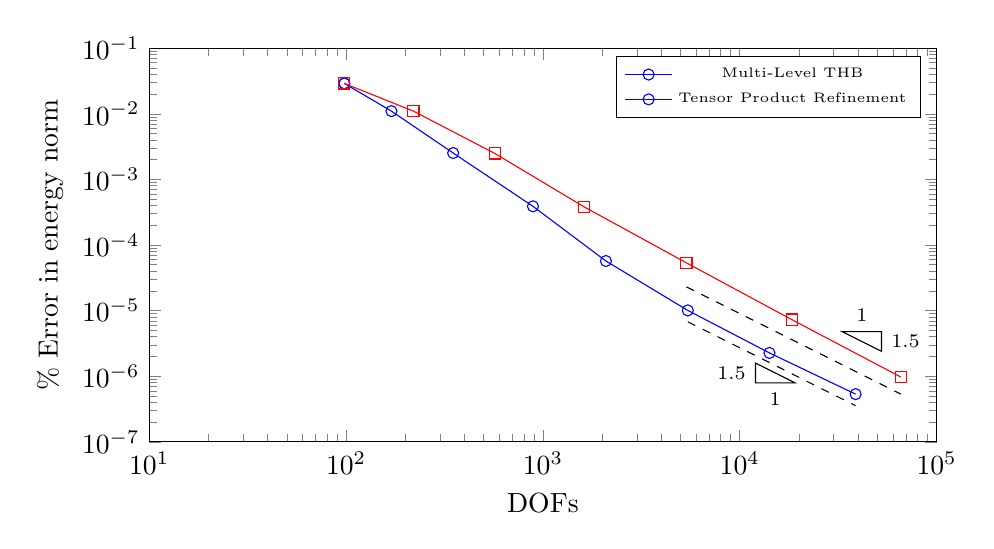
\begin{tikzpicture}

\begin{axis}[%
width=10cm,
height=5cm,
at={(0.758in,0.481in)},
scale only axis,
xmode=log,
xmin=1e1,
xmax=1e5,
xminorticks=true,
ymode=log,
ymin=1e-07,
ymax=0.1,
yminorticks=true,
axis background/.style={fill=white},
ylabel=\% Error in energy norm,
xlabel=DOFs,
legend style={font=\tiny}
]
%\addplot [color=blue,solid,mark=o,mark options={solid}]
\addplot [color=blue,solid,mark=o,mark options={solid}]
table[row sep=crcr]{%
	98	0.0290188281945\\
%	48	0.0500073829665119\\
%	76	0.0278449560820008\\
%	142	0.0126970619240542\\
%	242	0.00660733441696399\\
%	312	0.00435668459205658\\
%	552	0.00255759420607355\\
%	796	0.00151589672287713\\
%	1236	0.000944445092205633\\
%	2074	0.000566215208140263\\
%	3146	0.000339514546405781\\
%	4640	0.000241941547691511\\
%	8126	0.000134548935705695\\
%	11536	8.70810027272917e-05\\
%	16760	6.25408392329503e-05\\
};

\addplot [color=blue,solid,mark=o,mark options={solid}]
table[row sep=crcr]{%
	98	0.0290188281945\\
	170	0.01098025435962\\
	350	0.002524590268871\\
	890	0.000388921941731\\
	2090	5.7025394796e-05\\
	5446	1.0066756539e-05\\
	14156	2.266355311e-06\\
	38782	5.33491072e-07\\
};
\addplot [color=black,dashed,forget plot]
table[row sep=crcr]{%
%	98	0.0028019176590081\\
%	170	0.00122636881896947\\
%	350	0.00041513792990968\\
%	890	0.000102378667312402\\
%	2090	2.84495271636106e-05\\
	5446	6.76360172763725e-06\\
	14156	1.61392612232329e-06\\
	38782	3.55917366125145e-07\\
};

\addplot [color=red,solid,mark=square,mark options={solid}]
table[row sep=crcr]{%
	98	0.0290188281945\\
	220	0.010965623850222\\
	570	0.002484820200918\\
	1610	0.000385046254527\\
	5360	5.3462569201e-05\\
	18340	7.320546514e-06\\
	65786	9.72301108e-07\\
};
\addplot [color=black,dashed,forget plot]
table[row sep=crcr]{%
%	98	0.00930269423578717\\
%	220	0.00276575584547609\\
%	570	0.000663186346776017\\
%	1610	0.000139704065990453\\
	5360	2.29985616465477e-05\\
	18340	3.63369827887017e-06\\
	65786	5.34869260357945e-07\\
};


\legend{Multi-Level THB, Tensor Product Refinement}

{
\logLogSlopeReverseTriangle{0.77}{0.05}{0.15}{1.5}{black};
\logLogSlopeTriangle{0.93}{0.05}{0.28}{1.5}{black};
}
\end{axis}
\end{tikzpicture}%